\section{Summary of the Case Study}
In the case study, \citet{shaikh2023information} ask: ``How do cybersecurity breach costs and Top Management Team (TMT) attention to cybersecurity influence a firm's decision to carry out an Information Security Risk Assessment (ISRA)?''. The research found that higher breach costs result in greater TMT attention to cybersecurity. Additionally, they find that TMT attention to cybersecurity partially mediates the relationship between breach costs and the decision to conduct an ISRA. Further elaborating that while an ISRA might sometimes be initiated by the cybersecurity function independently, the TMT plays a significant role in the decision, especially after high-cost breaches.

\section{Explanation of the Attention-Based View (ABV) Theory}
The case study uses the attention-based view (ABV) to explain how TMT attention is directed toward cybersecurity issues. The ABV theory suggests that firm behaviour is shaped by how decision-makers allocate their attention. This theory is built on the idea that human rationality is limited, and decision-makers must focus on specific issues to make effective choices. The ABV is composed of three key principles: focus of attention, structural distribution of attention, and situated attention.

    \subsection{Focus of Attention}
    The principle of the focus of attention explains that due to limited attention capacity, individuals prioritise issues based on their perceived importance and relevance within a given context. Senior managers must be selective about which issues they focus on because they cannot effectively attend to everything. Negative events such as high-cost cybersecurity breaches become salient, thus requiring TMT attention. This focus then dictates the actions decision-makers take.

    \subsection{Structural Distribution of Attention}
    The principle of structural distribution of attention posits that an individual's position within an organisation's hierarchy influences what they pay attention to. TMTs have a fiduciary duty to stakeholders to oversee and assess firm performance and must protect the firm's reputation. As the ultimate decision-makers, they are responsible for oversight. The TMT's hierarchical position means they are expected to pay closer attention to security issues, especially in the face of higher breach costs.

    \subsection{Situated Attention}
    The principle of situated attention argues that an individual's attention is a result of the immediate situation. Urgent issues, such as high-cost cybersecurity breaches that cause material damage to the firm, draw the focus of the TMT. While minor breaches might be handled by IT personnel, breaches with substantial financial or reputational consequences require managerial attention and follow-up.

\section{Statement of Hypotheses}
The case study tested the following four hypotheses related to the impact of cybersecurity breach costs and TMT attention on the decision to carry out an ISRA:
\begin{enumerate}
    \item Higher cybersecurity breach costs have a positive effect on the decision to carry out an ISRA.
    \item Higher cybersecurity breach costs have a positive effect on TMT attention to cybersecurity.
    \item TMT attention to cybersecurity has a positive effect on the decision to carry out an ISRA.
    \item TMT attention to cybersecurity mediates the positive effect of cybersecurity breach costs on the decision to carry out an ISRA.
\end{enumerate}

\section{Critical Appraisal of the ABV}

    \subsection{Merits/Strengths}
    The Attention-Based View (ABV) provides a strong framework for understanding why Top Management Team (TMT) attention to cybersecurity is heightened following a costly breach. The ABV effectively explains this through its core principles: focus of attention, structural distribution of attention, and situated attention. The focus of attention principle highlights how negative events like significant breaches become salient, compelling the TMT to prioritise cybersecurity, while the structural distribution of attention principle emphasises that the TMT's hierarchical position and fiduciary duty make them responsible for addressing major security failures. Situated attention further reinforces this by illustrating how immediate, severe breaches demand urgent managerial action.

    The ABV also explains why some firms might not act on security until a crisis emerges. According to the model (see Figure \ref{fig:ABV}), TMTs have a limited attention capacity and will only focus on issues that are deemed the most important. This limited attention capacity means that cybersecurity may not receive sufficient attention until a significant breach forces the TMT to recognise it as a priority. This is further supported by the idea that organisations may only react to failures rather than carry out preventive security measures due to difficulty in justifying security investments. The ABV also theorises that breaches can act as a learning opportunity, as they provide inputs to enhance the quality of future security risk assessments.

    \begin{figure}[htbp]
        \centering
        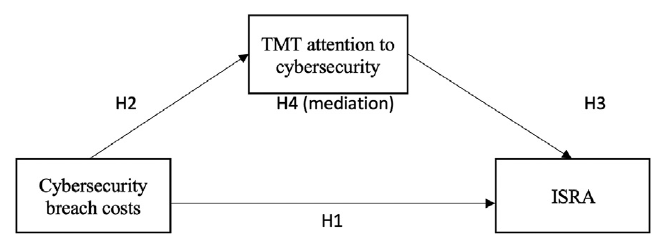
\includegraphics[width=0.8\textwidth]{figures/ABV-Theory.png}
        \caption{The Attention-Based View (ABV) Theory of TMT attention allocation, illustrating how breaches and organisational hierarchy influence decision-makers' focus \citep{shaikh2023information}.}
        \label{fig:ABV}
    \end{figure}

    \subsection{Demerits/Weaknesses}
    Despite its strengths, the ABV has some notable weaknesses. A significant limitation is that it primarily focuses on a reactive response to breaches, overlooking proactive security planning. The model is designed to explain how TMT attention is drawn to cybersecurity after a breach has occurred, but it does not adequately address how to prevent breaches in the first place. The ABV's emphasis on learning from failures shows its reactive stance, meaning that firms are continually playing catch up, rather than staying ahead of emerging threats.

    Additionally, the model assumes that TMT attention is driven primarily by negative events, ignoring other influences. While high-cost breaches undoubtedly capture the TMT's attention, \citet{gale2022governing} state that regulatory changes and industry standards are the most influential driver of board director's involvement in cybersecurity oversight. The ABV's narrow focus on breach-driven attention may lead to an incomplete understanding of the broader factors influencing security governance.

    Furthermore, the ABV does not provide a framework for proactive security measures. The model explains why TMTs react to breaches, but it offers little guidance on how to implement a security posture that anticipates threats. The model's focus on how the TMT reacts after a breach also overlooks the need for continuous monitoring, security by design, and other proactive strategies.

\section{Transition to New Model}
The limitations of the ABV indicate the need for a new, proactive model. While the ABV explains how firms respond to crises, a more comprehensive approach is required to prevent them. The next section will present a new model for information security risk assessment that shifts from a reactive to a proactive approach and addresses the limitations of the ABV. This new model is intended to help organisations implement security at every stage, rather than after they have already suffered a costly breach.